\documentclass{cumcm}
\usepackage{graphicx}
\usepackage{appendix}
\numberwithin{equation}{section}
\numberwithin{equation}{subsection}
\usepackage{csvsimple}
\usepackage{listings}
\usepackage{xcolor}
%\renewcommand{\baselinestretch}{1.0}
%\newcommand{\songtiB}

% \title{text}这里是显示在第三页的文章标题
\title{\textbf{计算机系统结构实验报告\quad 实验5}\\{\Large 类MIPS单周期处理器的设计与实现}}
\author{方泓杰\ 518030910150}


\begin{document}
\maketitle

\begin{abstract}
  本实验实现了类MIPS单周期处理器的几个重要部件,该类MIPS单周期处理器的CPU支持16条MIPS指令(包括R型指令中的add、sub、and、or、slt、sll、srl、jr;I型指令中的lw、sw、addi、ori、beq;J型指令中的j、jal)。本实验以实验三、四实现的模块为基础,对部分功能进行了修改,同时添加了部分控制信号。本实验通过软件仿真的形式进行实验结果的验证。
\end{abstract}

\maketitle \tableofcontents
\newpage

\section{实验目的}\label{section1}
本次实验有如下三个实验目的:
\begin{enumerate}
    \item 理解类MIPS单周期处理器的工作原理;
    \item 对类MIPS单周期处理器的各个子模块与顶层模块的设计与调试;
    \item 使用功能仿真验证功能实现的正确性。
\end{enumerate}

\section{原理分析}\label{section2}

\subsection{主控制器(Ctr)原理分析}\label{section2.1}
主控制器需要对指令的最高6位的OpCode域进行解析,初步判断指令的类型并产生对应的处理器控制信号。我们在主控制器中将指令的类型做如下区分:R型指令(具体的指令在这里不做区分,留给运算单元控制器(ALUCtr)区分);I型指令中的load指令(lw),store指令(sw)与branch指令(beq);J型指令中的jump指令(j, jal)。本次实验中用到的控制信号如表 \ref{tab1} 所示。

\begin{table}[htbp]
    \centering
    \begin{tabular}{|c|c|}
         \hline
         信号 & 具体说明 \\ \hline
         ALUSrc & 算术逻辑运算单元(ALU)的第二个操作数的来源(0:使用rt;1:使用立即数)\\
         ALUOp (*) & 发送给运算单元控制器(ALUCtr)用来进一步解析运算类型的控制信号 \\
         Branch & 条件跳转信号,高电平说明当前指令是条件跳转指令(branch) \\
         extSign & 符号扩展信号,高电平说明当前指令需要进行符号拓展 \\
         JalSign & jal指令信号,高电平说明当前指令是jal指令 \\
         Jump & 无条件跳转信号,高电平说明当前指令是无条件跳转指令(jump) \\
         memRead & 内存读使能信号,高电平说明当前指令需要进行内存读取(load) \\
         memToReg & 写寄存器的数据来源 (0:使用ALU运算结果;1:使用内存读取数据) \\
         memWrite & 内存写使能信号,高电平说明当前指令需要进行内存写入(store) \\
         regDst & 目标寄存器的选择信号(0:写入rt代表的寄存器;1:写入rd代表的寄存器)\\
         regWrite & 寄存器写使能信号,高电平说明当前指令需要进行寄存器写入 \\
         \hline
    \end{tabular}
    \caption{主控制器产生的控制信号}
    \label{tab1}
\end{table}

上表中标(*)的ALUOp信号包含三个二进制位,所代表的具体含义以及解析方式如表 \ref{tab2} 所示。

\begin{table}[htbp]
    \centering
    \begin{tabular}{|c|c|c|}
         \hline
         ALUOp的信号内容 & 指令 & 具体说明 \\
         \hline
         000 / 010 & lw, sw / addi & ALU执行加法运算 \\
         001 & beq & ALU执行减法运算 \\
         011 & andi & ALU执行逻辑与运算 \\
         100 & ori & ALU执行逻辑或运算 \\
         101 & R型指令 & ALU具体执行内容需要根据指令最后6位的Funct域决定 \\
         110 & j, jal & ALU不需要进行操作 \\
         \hline
    \end{tabular}
    \caption{ALUOp信号的具体含义以及解析方式}
    \label{tab2}
\end{table}

从表 \ref{tab2} 中我们可以发现,ALUOp实际上相当于在主控制器(Ctr)中预先得出的部分非R型指令(如beq指令、j指令、lw指令以及sw指令等)的ALU控制信号;例如当前指令为beq指令,那么ALU实际需要执行的运算为减法,于是ALUOp信号为01,表示ALU应该执行减法操作。当然该控制信号并不能直接送入ALU,还需要经过运算单元控制器(ALUCtr)进行进一步的处理,得到最终的运算单元控制信号ALUCtrOut,之后才能送入ALU进行对其的控制。

注意到,我们在实验三的基础上增添了许多新的信号,也增加了ALUOp的位数支持新加入的里技术类性指令(由于这些指令的运算包含在OpCode中,所以我们必须提前解析)。

因篇幅所限,这里不再列出主控制器(Ctr)产生的各种控制信号与指令OpCode域的对应方式;可以参照指令的含义以及表 \ref{tab1} 所示的信号含义进行解析,方法与实验三时所用的方法相同。当出现其他暂不支持的指令时,我们将所有的控制信号均置为0,将这条指令看作一条空指令(nop),使得该指令对数据没有影响,保证数据的正确性。

\subsection{运算单元控制器(ALUCtr)原理分析}\label{section2.2}

运算单元控制器(ALUCtr)对指令的最后6位的Funct域进行解析,结合主控制器(Ctr)产生的ALUOp信号,给出最终的运算单元控制信号ALUCtrOut。该信号作用于ALU,实现对于ALU不同功能的控制。运算单元控制器(ALUCtr)的解析方式如表 \ref{tab4} 所示。

\begin{table}[htbp]
    \centering
    \begin{tabular}{|c|c|c|c|c|}
        \hline
        指令 & ALUOp & Funct & ALUCtrOut & 具体说明\\ \hline
        lw & 000 & xxxxxx & 0010 & ALU执行加法运算 \\
        sw & 000 & xxxxxx & 0010 & ALU执行加法运算 \\
        beq & 001 & xxxxxx & 0110 & ALU执行减法运算 \\
        addi & 010 & xxxxxx & 0010 & ALU执行加法运算 \\
        andi & 011 & xxxxxx & 0000 & ALU执行逻辑与运算 \\
        ori & 100 & xxxxxx & 0001 & ALU执行逻辑或运算 \\
        sll & 101 & 000000 & 0011 & ALU执行逻辑左移运算 \\
        srl & 101 & 000010 & 0100 & ALU执行逻辑右移运算 \\
        jr & 101 & 001000 & 0101 & ALU不用进行运算 \\
        add & 101 & 100000 & 0010 & ALU执行加法运算 \\
        sub & 101 & 100010 & 0110 & ALU执行减法运算 \\
        and & 101 & 100100 & 0000 & ALU执行逻辑与运算 \\
        or & 101 & 100101 & 0001 & ALU执行逻辑或运算 \\
        slt & 101 & 101010 & 0111 & ALU执行小于时置位运算 \\
        j & 110 & xxxxxx & 0101 & ALU不用进行运算 \\
        jal & 110 & xxxxxx & 0101 & ALU不用进行运算 \\
        \hline
    \end{tabular}
    \caption{运算单元控制器(ALUCtr)的解析方式}
    \label{tab3}
\end{table}

从表 \ref{tab3} 中可以看出,运算单元控制信号ALUCtrOut与ALU执行的操作类型有一一对应的关系,我们将在第 \ref{section2.3} 节给出具体的对应方式。此外,为了支持jr指令以及带有shamt操作数的sll与srl指令,我们新增了两个信号jrSign与shamtSign,分别用来表示该指令是否为jr、该指令操作数是否在shamt中。这两个信号将会在指令解析完成后进行处理。

\subsection{算术逻辑运算单元(ALU)原理分析}\label{section2.3}

ALU主要根据由运算单元控制器(ALUCtr)产生的运算单元控制信号ALUCtrOut,对输入的两个数执行对应的算术逻辑运算,输出运算的结果以及部分控制信号。其输出的一个重要信号为 zero 信号,当运算结果为 0 时该信号为高电平,否则为低电平;该信号用于与 branch 指令结合判断是否满足转移条件。ALU执行的算术逻辑运算类型与运算单元控制信号ALUCtrOut的对应方式如表 \ref{tab4} 所示。

\begin{table}[htbp]
    \centering
    \begin{tabular}{|c|c|}
         \hline
         ALUCtrOut & ALU执行算术逻辑运算类型 \\
         \hline
         0000 & 逻辑与 (and) \\
         0001 & 逻辑或 (or) \\
         0010 & 加法 (add) \\
         0011 & 左移 (left-shift) \\
         0100 & 右移 (right-shift) \\
         0101 & 无运算 (nop) \\
         0110 & 减法 (sub) \\
         0111 & 小于时置位 (slt) \\
         \hline
    \end{tabular}
    \caption{ALU执行的算术逻辑运算类型与ALUCtrOut的对应方式}
    \label{tab4}
\end{table}

\subsection{寄存器(Register)原理分析}\label{section2.4}

本部分和实验四的寄存器的原理分析完全相同,不再赘述。

\subsection{存储器(Data Memory)原理分析}\label{section2.5}

本部分和实验四的存储器的原理分析完全相同,不再赘述。

\subsection{指令存储器(Instruction Memory)原理分析}\label{section2.6}

本部分和第 \ref{section2.5} 节中的存储器几乎相同,而且不需要支持修改操作。因此在读入初始数据后,后续只要直接输出给定的输入PC值所指向的指令即可。

\subsection{有符号扩展单元(Sign Extension)原理分析}\label{section2.7}

本部分和实验四的有符号扩展单元的原理分析完全相同,不再赘述。

\subsection{数据选择器(Mux)原理分析}\label{section2.8}

数据选择器的主要原理是根据指定信号,选择两个输入数据通路的其中对应的一个输出。包括两种数据选择器,一种的输入输出均为5位数据通路,一种输入输出均为32位数据通路,可按需选用。

\subsection{程序计数器模块(PC)原理分析}\label{section2.9}

程序计数器模块的主要原理是在时钟上升沿(一个周期的开始)将PC进行修改后输出,我们设计了一个模块来进行实现。实际上,在后面实验六的操作中我们发现,可以直接使用非阻塞赋值实现。但是这里我们仍然采用模块化的设计方法,便于整个处理器的调试。

\subsection{顶层模块(Top)原理分析}\label{section2.10}
顶层模块的实现主要是将第 \ref{section2.1} 节至第 \ref{section2.9} 节中描述的所有模块实例化并组装而成,这里给出整体组装后的单周期MIPS处理器的电路设计图,如图 \ref{fig1} 所示。

\begin{figure}[htbp]
    \centering
    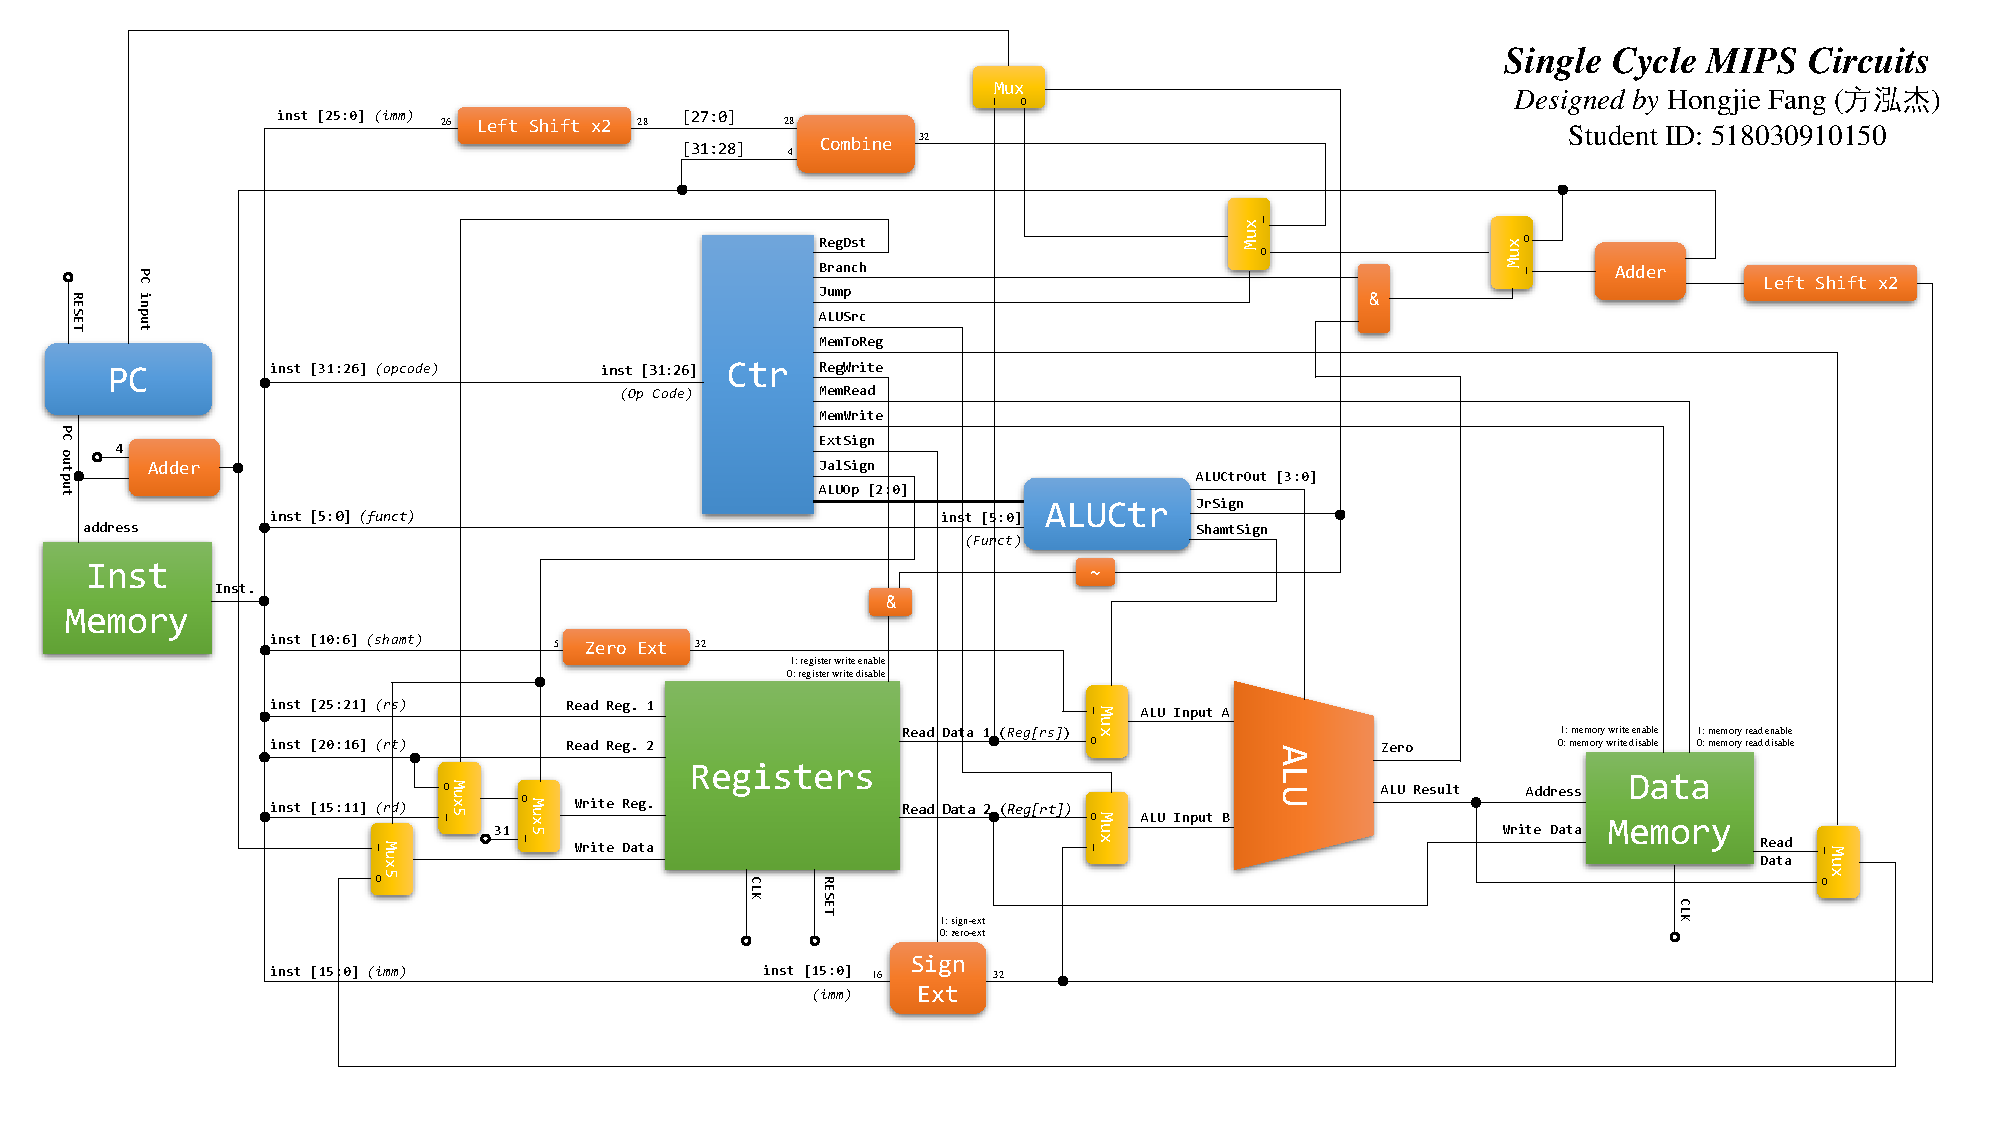
\includegraphics[width=7in]{Design.pdf}
    \caption{单周期MIPS处理器电路设计图}
    \label{fig1}
\end{figure}

\section{功能实现}\label{section3}
\subsection{主控制器(Ctr)功能实现}\label{section3.1}

在第 \ref{section2.1} 节中我们详细介绍了主控制器(Ctr)的设计,我们只需要按照设计的信号进行相应的实现即可。在这里我们使用了Verilog中的\texttt{case}语句进行实现,下面\textbf{节选部分代码进行展示},完整代码详见附录 \ref{appsection1.1}。注意,这里的\texttt{default}选项表示出现不支持指令时,我们将其当作一条空指令(nop)进行处理,对数据不产生影响。

\begin{lstlisting}[language=verilog]
always @(opCode)
    begin
        case(opCode)
            6'b000000:      // R Type
            begin
                regDst = 1;
                aluSrc = 0;
                memToReg = 0;
                regWrite = 1;
                memRead = 0;
                memWrite = 0;
                branch = 0;
                extSign = 0;
                jalSign = 0;
                aluOp = 3'b101;
                jump = 0;
            end
            6'b100011:      // lw
            begin
                regDst = 0;
                aluSrc = 1;
                memToReg = 1;
                regWrite = 1;
                memRead = 1;
                memWrite = 0;
                branch = 0;
                extSign = 1;
                jalSign = 0;
                aluOp = 3'b000;
                jump = 0;
            end
            // ......
            default:        // default
            begin
                regDst = 0;
                aluSrc = 0;
                memToReg = 0;
                regWrite = 0;
                memRead = 0;
                memWrite = 0;
                branch = 0;
                extSign = 0;
                jalSign = 0;
                aluOp = 3'b111;
                jump = 0;
            end
        endcase
    end
\end{lstlisting}

注意到当出现不支持的指令时,我们将ALUOp信号设为111,表示未定义的操作,同时将其他的所有控制信号置零,这样在后续过程中不会进行任何操作。

\subsection{运算单元控制器(ALUCtr)功能实现}\label{section3.2}

在第 \ref{section2.2} 节中我们详细介绍了运算单元控制器(ALUCtr)的设计,我们只需要按照第 \ref{section2.2} 节中的表 \ref{tab3} 进行相应信号的实现即可。在这里我们使用了Verilog中的\texttt{casex}语句(即带通配符\texttt{x}的\texttt{case}语句)进行实现,\underline{下面节选部分代码进行展示},完整代码详见附录 \ref{appsection1.2}。

\begin{lstlisting}[language=verilog]
always @ (aluOp or funct)
    begin
        casex ({aluOp, funct})
            9'b000xxxxxx:  // lw or sw: actually add
                aluCtrOut = 4'b0010;
            9'b001xxxxxx:  // beq: actually sub
                aluCtrOut = 4'b0110;
            // ...... 
            9'b101101010:  // slt: actually set on less than
                aluCtrOut = 4'b0111;
            9'b110xxxxxx:  // jump / jal: actually not change
                aluCtrOut = 4'b0101;
        endcase        
        
        if ({aluOp, funct} == 9'b101000000 || {aluOp, funct} == 9'b101000010)
            shamtSign = 1;
        else 
            shamtSign = 0;
        
        if ({aluOp, funct} == 9'b101001000)
            jrSign = 1;
        else 
            jrSign = 0;
    end
\end{lstlisting}

注意到我们在执行指令的进一步解析时,顺带产生了两个控制信号,分别是用于控制操作数是否从shamt中选取的shamtSign信号以及指令是否为jr的jrSign信号。

\subsection{算术逻辑运算单元(ALU)功能实现}\label{section3.3}

在第 \ref{section2.3} 节中我们详细介绍了运算单元控制器(ALUCtr)的设计,我们只需要按照第 \ref{section2.3} 节中的表 \ref{tab4} 进行相应信号的实现即可。在这里我们使用了Verilog中的\texttt{case}语句进行实现,同时在求出运算结果后进行\texttt{zero}信号的设置。代码部分和实验三的非常类似,在此不再展示,完整代码可参考附录 \ref{appsection1.3}。

\subsection{寄存器(Register)功能实现}\label{section3.4}
寄存器的实现与实验四中实现的寄存器几乎完全相同,在此不再赘述,完整代码可参考附录 \ref{appsection1.4}。

\subsection{存储器(Data Memory)功能实现}\label{section3.5}
存储器的实现与实验四中实现的存储器几乎完全相同,在此不再赘述,完整代码可参考附录 \ref{appsection1.5}。

\subsection{指令存储器(Instruction Memory)功能实现}\label{section3.6}
指令存储器的实现与存储器十分类似,且其不需要支持修改操作,因此可以利用存储器的代码稍加修改得出,在此不再赘述,完整代码可参考附录 \ref{appsection1.6}。

\subsection{有符号拓展单元(Sign Extension)功能实现}\label{section3.7}
有符号扩展单元的实现与实验四中实现的有符号扩展单元几乎完全相同,在此不再赘述,完整代码可参考附录 \ref{appsection1.7}。

\subsection{数据选择器(Mux)功能实现}\label{section3.8}
在第 \ref{section2.8} 节中我们详细介绍了数据选择器(Mux),其分为5位数据选择器与32位数据选择器;以32位数据选择器为例,我们通过条件三目运算符代替\texttt{if}语句进行实现。在此展示32位数据选择器的部分代码,两类数据选择器的完整代码可参考附录 \ref{appsection1.8}。
\begin{lstlisting}[language=verilog]
module Mux(
    input selectSignal,
    input [31 : 0] input1,
    input [31 : 0] input2,
    output [31 : 0] out
    );
    assign out = selectSignal ? input1 : input2;
endmodule
\end{lstlisting}

\subsection{程序计数器模块(PC)功能实现}\label{section3.9}
在第 \ref{section2.9} 节中我们详细介绍了程序计数器模块(PC),我们在此利用模块进行实现,下面节选部分代码进行展示,完整的代码可参考附录 \ref{appsection1.9}。
\begin{lstlisting}[language=verilog]
always @ (posedge clk or reset)
    begin
        if (reset)
            pcOut = 0;
        else
            pcOut = pcIn;
        $display("PC: %d\n", pcOut);
    end
\end{lstlisting}

注意到,我们在代码最后加入了显示当前PC的指令,以方便后续的调试以及结果的验证。

\subsection{顶层模块(Top)功能实现}\label{section3.10}

在第 \ref{section2.10} 节中我们详细介绍了顶层模块(Top),我们根据图 \ref{fig1} 中的连线,定义如下数据线(每一条线都对应着图中的一条线)。

\begin{lstlisting}[language=verilog]
    wire [31 : 0] INST_ADDR;        // INSTRUCTION ADDRESS
    wire [31 : 0] INST;             // INSTRUCTION
    wire REG_DST;                   // REG DST
    wire ALU_SRC;                   // ALU SRC
    wire MEM_TO_REG;                // MEM TO REG
    wire REG_WRITE;                 // REG WRITE
    wire MEM_READ;                  // MEM READ
    wire MEM_WRITE;                 // MEM WRITE
    wire BRANCH;                    // BRANCH
    wire EXT_SIGN;                  // EXT SIGN
    wire JAL_SIGN;                  // JAL SIGN
    wire [2 : 0] ALU_OP;            // ALU OP
    wire JUMP;                      // JUMP
    wire [3 : 0] ALU_CTR_OUT;       // ALU CTR OUT
    wire SHAMT_SIGN;                // SHAMT SIGN
    wire JR_SIGN;                   // JR SIGN
    wire [31 : 0] REG_OUT1;         // REG OUTPUT 1 (rs)
    wire [31 : 0] REG_OUT2;         // REG OUTPUT 2 (rt)
    wire [31 : 0] ALU_INPUT_A;      // ALU INPUT A
    wire [31 : 0] ALU_INPUT_B;      // ALU INPUT B
    wire [31 : 0] EXT_RES;          // EXT RESULT
    wire ALU_OUT_ZERO;              // ALU OUT ZERO
    wire [31 : 0] ALU_RES;          // ALU RESULT  
    wire [4 : 0] READ_REG1;         // READ REG 1
    wire [4 : 0] READ_REG2;         // READ REG 2
    wire [4 : 0] WRITE_REG;         // WRITE REG
    wire [31 : 0] REG_WRITE_DATA;   // REG WRITE DATA
    wire [31 : 0] REG_WRITE_DATA_T; // REG WRITE DATA TEMP
    wire [4 : 0] WRITE_REG_TEMP;    // WRITE REG TEMP
    wire [31 : 0] PC_IN;            // PC INPUT
    wire [31 : 0] PC_OUT;           // PC OUTPUT
    wire [31 : 0] MEM_READ_DATA;    // MEM READ DATA
    wire [31 : 0] PC_TEMP1;         // PC TEMP1
    wire [31 : 0] PC_TEMP2;         // PC TEMP2
\end{lstlisting}

接着,我们利用第 \ref{section3.1} 节至第 \ref{section3.9} 节中实现好的模块,将上述连线连入模块的对应输入/输出端。以主控制器为例,将对应的指令的opCode域连入主控制器的opCode输入端,并将其产生的控制信号连入主控制器对应的控制信号输出端即可。下面展示主控制器的部分代码,完整代码参见附录 \ref{appsection1.10}。

\begin{lstlisting}[language=verilog]
    Ctr main_controller (
        .opCode(INST[31 : 26]),
        .regDst(REG_DST),
        .aluSrc(ALU_SRC),
        .memToReg(MEM_TO_REG),
        .regWrite(REG_WRITE),
        .memRead(MEM_READ),
        .memWrite(MEM_WRITE),
        .branch(BRANCH),
        .extSign(EXT_SIGN),
        .jalSign(JAL_SIGN),
        .aluOp(ALU_OP),
        .jump(JUMP)
    );
\end{lstlisting}

\section{结果验证}\label{section4}
我们首先在内存中载入如下初始值。

\begin{table}[htbp]
    \centering
    \begin{tabular}{|c|c|c|c|c|}
        \hline
        地址 & 数据(十六进制) & 地址 & 数据(十六进制)\\ \hline
        1 & 000000FF & 
        2 & 00000100\\
        3 & 00000101 & 
        4 & 00000102\\
        5 & 00000000 &
        6 & 00000001\\
        7 & 00000002 &
        8 & 00000003\\
        9 & 00000004 &
        10 & 00000005\\
        11 & 00000006 &
        12 & 00000007\\
        13 & 00000103 &
        14 & 00000104\\
        15 & 00000105 &
        16 & 00000106\\
        17 & 00000008 &
        18 & 00000009\\
        19 & 0000000A &
        20 & 00000107\\
        21 & 00000108 &
        22 & 00000109\\
        23 & 0000010A &
        24 & 000001FF\\
        25 & 000002FF &
        26 & 000003FF\\
        27 & 000004FF &
        28 & 000005FF\\
        29 & 000006FF &
        30 & 000007FF\\
        31 & 000008FF &
        32 & 000009FF\\
        \hline
    \end{tabular}
    \caption{内存中的初始值}
    \label{tab5}
\end{table}

我们在激励文件中使用readmemh命令将其读入存储器模块的对应位置进行测试。
\begin{lstlisting}[language=verilog]
$readmemh("C:/ArchLabs/CS145-ArchLabs/lab05/data.dat", processor.data_memory.memFile);         
\end{lstlisting}

接着,我们设计了如下汇编代码进行测试。


\begin{table}[htbp]
    \centering
    \begin{tabular}{|c|c|c|c|c|}
        \hline
        指令地址(line) & 指令 & 指令解释 & 执行结果\\ \hline
        0 & 100011 00000 00001 0000000000000000 & lw \$1, 0(\$0) & \$1 = Mem[0] = 255 \\
        1 & 100011 00000 00010 0000000000000001 & lw \$2, 1(\$0) & \$2 = Mem[1] = 256 \\
        2 & 100011 00000 00011 0000000000000111 & lw \$3, 7(\$0) & \$3 = Mem[7] = 3\\
        3 & 100011 00011 00100 0000000000001011 & lw \$4, 11(\$3) & \$4 = Mem[14] = 261\\
        4 & 000000 00001 00010 00110 00000 100000 & add \$6, \$1, \$2 & \$6 = 255 + 256 = 511\\
        5 & 000000 00100 00001 00111 00000 100010 & sub \$7, \$4, \$1 & \$7 = 261 – 255 = 6\\
        6 & 100011 00111 10000 0000000000000101 & lw \$16, 5(\$7) & \$16 = Mem[11] = 7\\
        7 & 000000 00001 00100 00101 00000 100100 & and \$5, \$1, \$4 & \$5 = 255 \& 261 = 5\\
        8 & 000000 10000 00010 01000 00000 100101 & or \$8, \$16, \$2 & \$8 = 7 | 256 = 263\\
        9 & 101011 00101 01000 0000000000000111 & sw \$8, 7(\$5) & Mem[12] = 263\\
        10 & 001000 00001 01010 0000000100000000 & addi \$10, \$1, 256 & \$10 = 255 + 256 = 511\\
        11 & 001100 00100 01011 0000000011111111 & andi \$11, \$4, 255 & \$11 = 261 \& 255 = 5\\
        12 & 001101 10000 01100 0000000100000000 & ori \$12, \$16, 256 & \$12 = 7 | 256 = 263\\
        13 & 100011 00000 01001 0000000000001100 & lw \$9, 12(\$0) & \$9 = Mem[12] = 263;\\
        14 & 000100 01001 01000 0000000000000001 & beq \$9, \$8, 1 & go to line 16;\\
        15 & 000000 00000 01011 01101 00100 000000 & sll \$13, \$11, 4 & (not executed)\\
        16 & 000000 00000 01011 01110 00100 000000 & sll \$14, \$11, 4 & \$14 = \$11 << 4 = 80\\
        17 & 000000 00000 01010 01111 00100 000010 & srl \$15, \$10, 4 & \$15 = \$10 >> 4 = 31\\
        18 & 000000 01111 01110 10001 00000 101010 & slt \$17, \$15, \$14 & \$17 = 1\\
        19 & 000000 01111 10000 10010 00000 101010 & slt \$18, \$15, \$16 & \$18 = 0\\
        20 & 000010 00000000000000000000010110 & j 22 & go to line 22\\
        21 & 000000 01111 01110 10010 00000 101010 & slt \$18, \$15, \$14 & (not executed) \\
        22 & 000011 00000000000000000000011000 & jal 24 & go to line 24\\
        23 & 000100 10000 01011 0000000000000011 & beq \$16, \$11, 3 & go to line 27;\\
        24 & 001000 01011 01011 0000000000000010 & addi \$11, \$11, 2 & \$11 = \$11 + 2 = 7\\
        25 & 000000 11111 00000 00000 00000 001000 & jr \$31 & go to line 23\\
        26 & 001000 01011 01011 0000000000000010 & addi \$11, \$11, 2 & (not executed)\\
        27 & 001000 01011 01011 0000000000000010 & addi \$11, \$11, 2 & \$11 = \$11 + 2 = 9\\
        \hline
    \end{tabular}
    \caption{汇编代码及其解释、执行结果}
    \label{tab6}
\end{table}

其中,执行结果中表明 “(not executed)” 表示该指令由于跳转等原因没有被执行。可以看出,我们的测试汇编代码完整测试了本实验要求的所有的16条汇编指令,因此该测试结果能够反映出处理器的整体实现准确与否。

类似地,我们在激励文件中用readmemb命令将其读入指令存储器模块的对应位置进行测试。
\begin{lstlisting}[language=verilog]
$readmemb("C:/ArchLabs/CS145-ArchLabs/lab05/inst_data.dat", processor.inst_memory.instFile);
\end{lstlisting}

\clearpage

我们用上述汇编命令以及内存的初始情况进行测试,测试结果如图 \ref{fig2} 所示。

\begin{figure}[htbp]
    \centering
    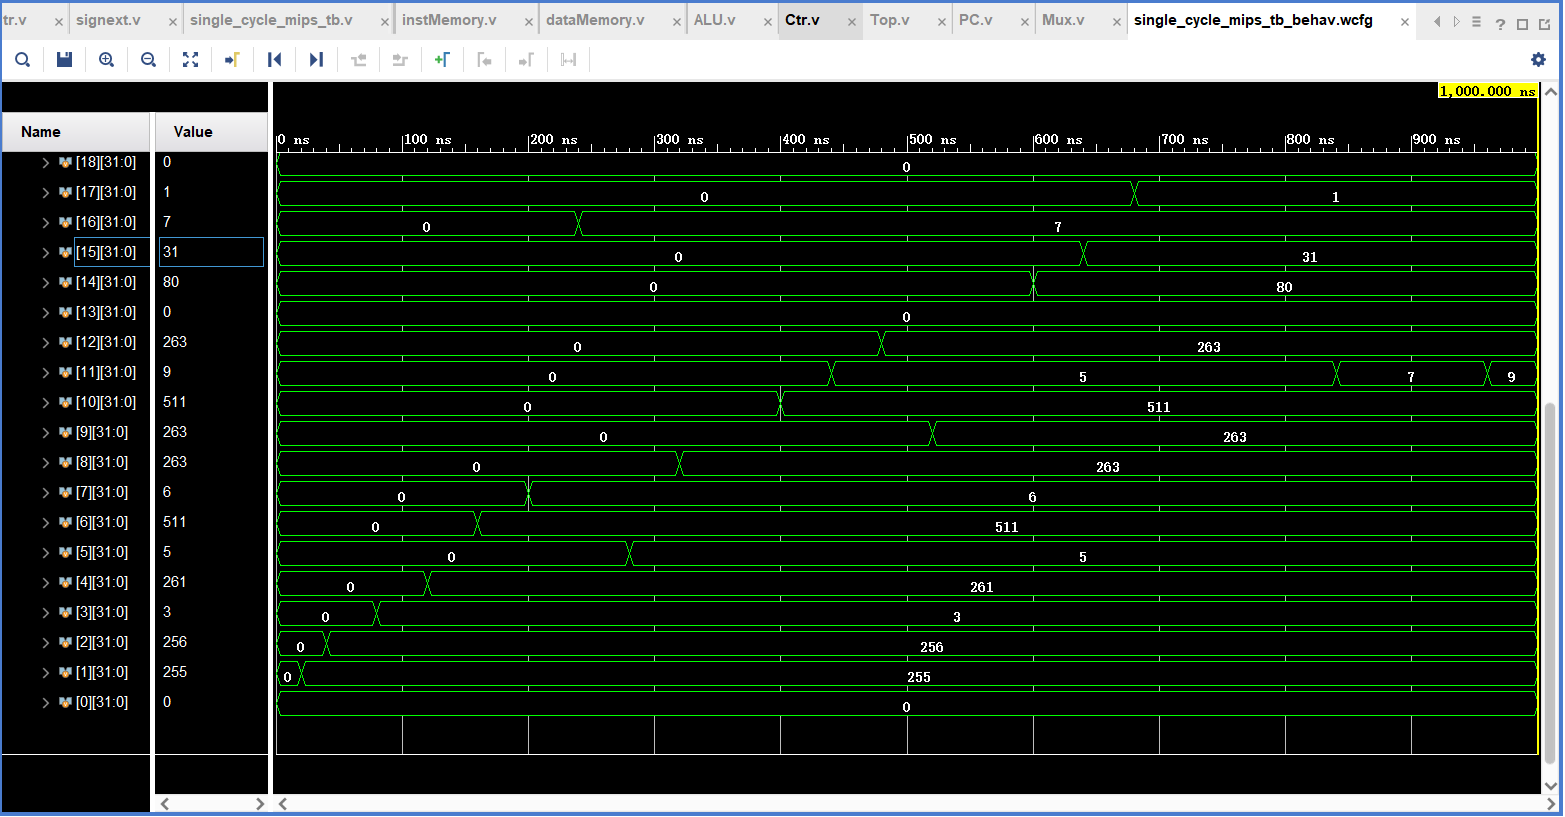
\includegraphics[width=7in]{1.png}
    \caption{单周期MIPS处理器测试结果}
    \label{fig2}
\end{figure}

对照图 \ref{fig2} 与表 \ref{tab6} 中的执行结果可知,运行结果完全正确,仿真成功,说明整个单周期MIPS处理器实现正确。

为了进一步说明我们实现的正确性,我添加了部分代码,在输出框中进行测试。首先我们来看一下测试jal与jr指令的片段(指令地址22至25的部分,line 22至line 25)。

\begin{figure}[htbp]
    \centering
    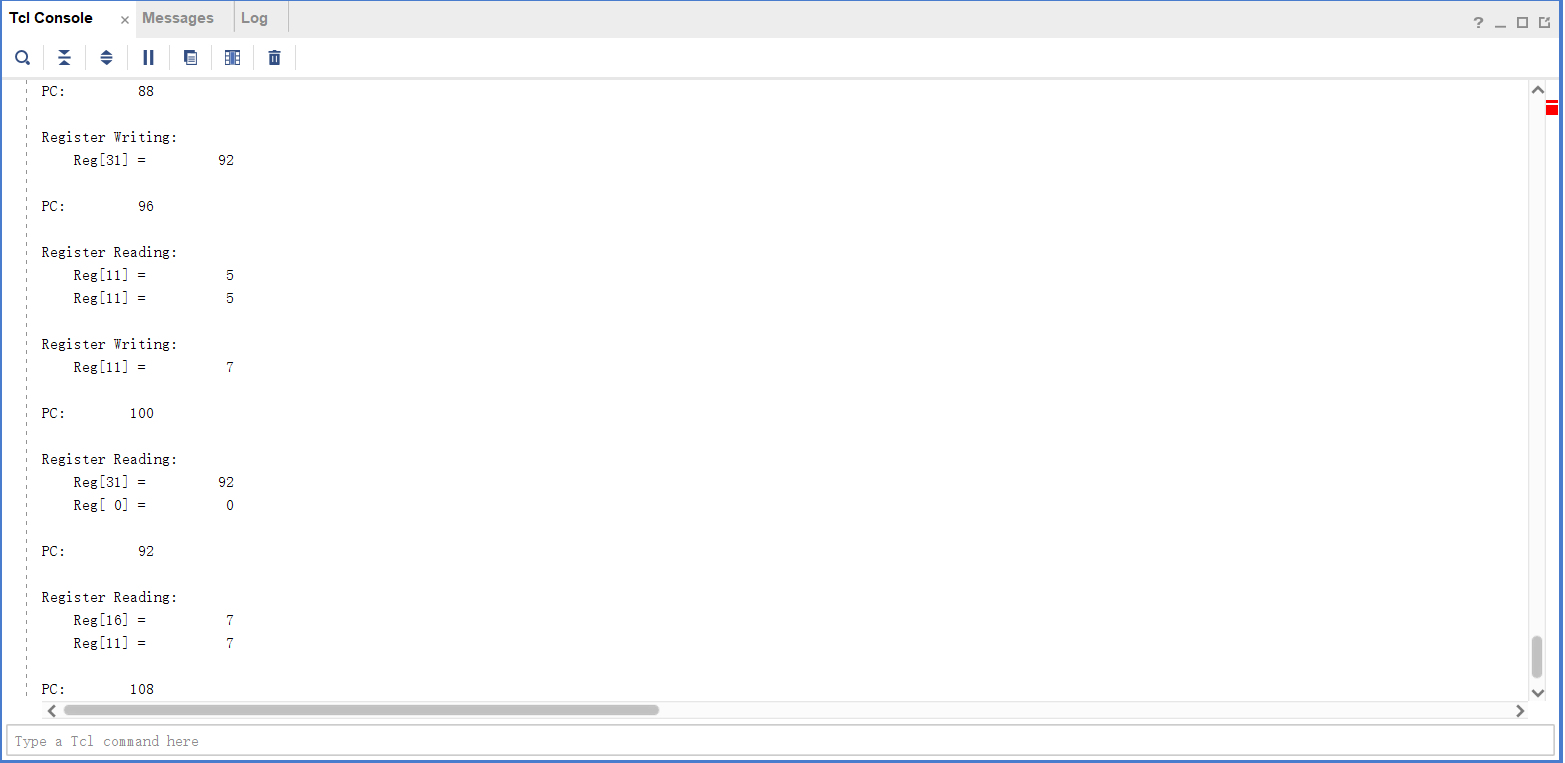
\includegraphics[width=6in]{2-jal-jr.png}
    \caption{单周期MIPS处理器的jal、jr指令的测试片段}
    \label{fig3}
\end{figure}

从图 \ref{fig3} 中可以看到,在指令地址22(此时PC为88)的jal指令时,我们向31号寄存器写入PC+4,即92,并跳转到指令地址24(此时PC为98);在执行指令地址25(此时PC为100)的jr指令时,我们没有修改任何信息,直接返回到了指令地址23(此时PC为92)。从这可以看出,jal与jr指令实现正确。

\clearpage 
接着,我们再来看测试beq指令的片段(指令地址23,line 23)。

\begin{figure}[htbp]
    \centering
    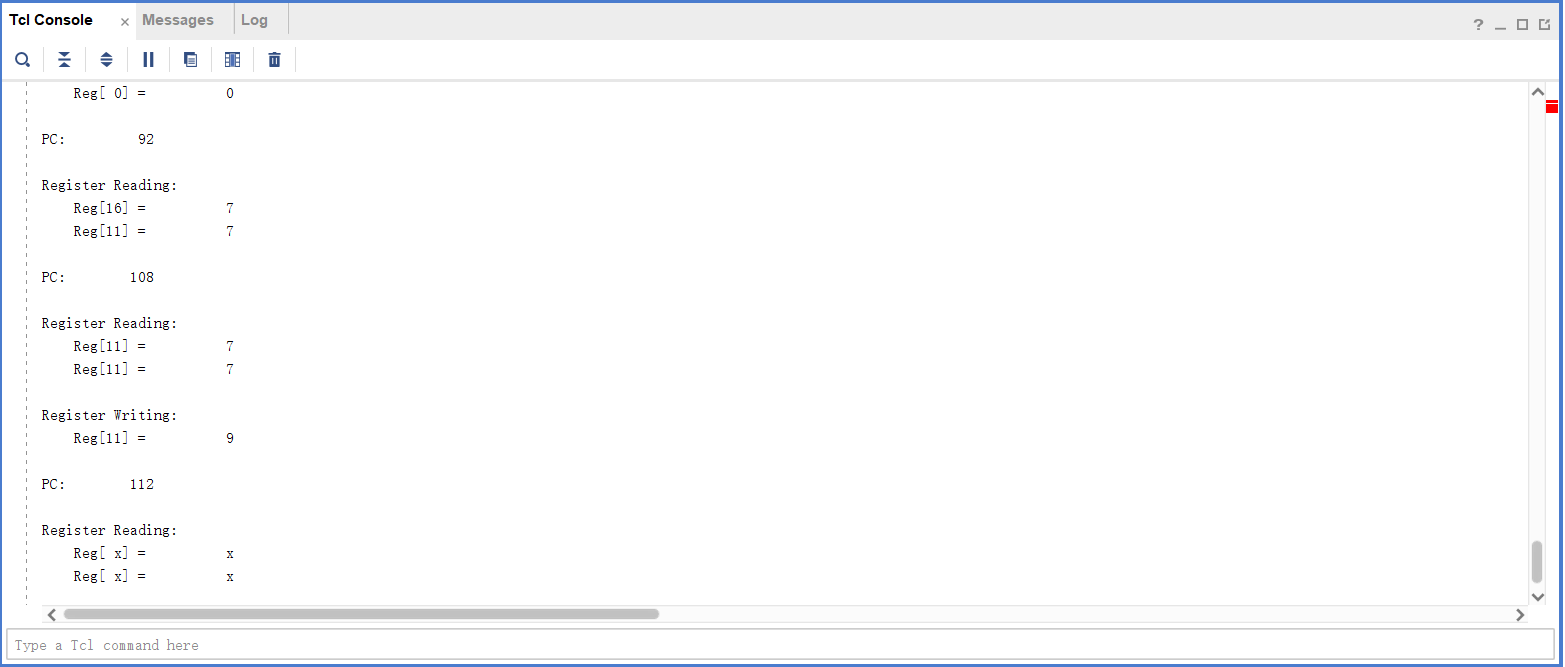
\includegraphics[width=6in]{3-beq.png}
    \caption{单周期MIPS处理器的beq指令的测试片段}
    \label{fig4}
\end{figure}

从图 \ref{fig4} 中可以看到,在指令地址23(此时PC为92)的beq指令时,由于两个寄存器数值相等均为7,我们跳转到了指令地址27(此时PC为108)的addi指令。从这可以看出,beq指令实现正确。

最后,我们来看一下测试j指令的片段(指令地址20,line 20)。

\begin{figure}[htbp]
    \centering
    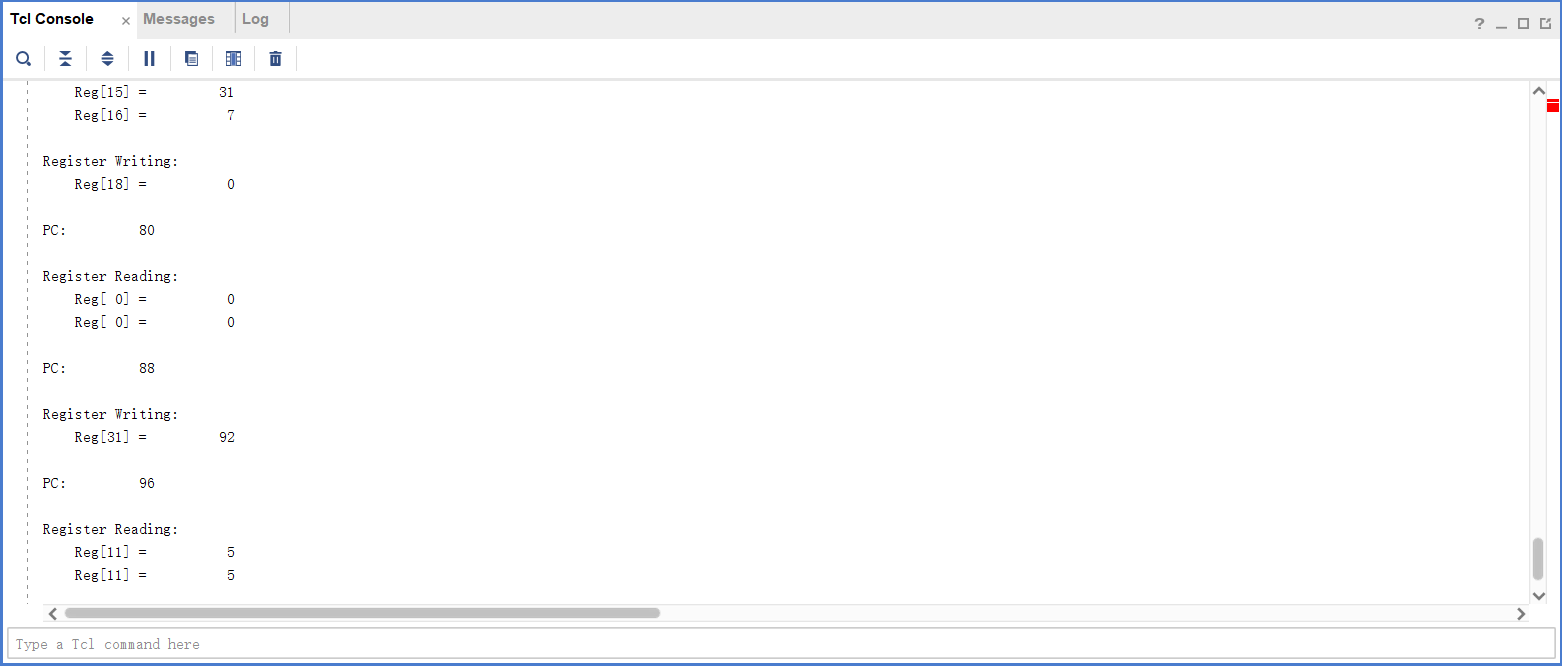
\includegraphics[width=6in]{4-j.png}
    \caption{单周期MIPS处理器的j指令的测试片段}
    \label{fig5}
\end{figure}

从图 \ref{fig5} 中可以看到,在指令地址20(此时PC为80)的j指令时,我们直接跳转到了指令地址22(此时PC为88)。从这里可以看出,j指令实现正确。

综上,经过详尽的测试,我们可以得出结论,我们的单周期MIPS处理器实现正确。

\section{总结与反思}\label{section5}

本实验实现了一个完整的支持16指令的单周期MIPS处理器,以实验三、四的模块为基础,添加部分其他模块后,将模块连线组装成一个完整的单周期MIPS处理器。通过这次实验,我对于MIPS处理器的数据通路、信号通路等都有了一个更加清晰地了解,也对单周期MIPS有了更加深刻的理解。同时,在实验时,我发现将完整的电路图(如图 \ref{fig1} 所示)画出有助于设计、检查、调试连线;因此,在之后的处理器设计中,在遇到调试困难时,将完整电路图(或部分部件的完整电路图)画出,不失为一种好的调试方法。

同时,在调试的过程中,我对MIPS处理器的指令也有了更加深刻的理解;通过自行编写对应的汇编代码、手动模拟汇编代码的运行结果、与自己写的处理器的运行结果进行对照等过程,对汇编代码也有了更加深刻的理解。同时,我认为设计出一个能够完整测试16指令的汇编代码也是一个比较繁琐的事情(特别是需要手动模拟、转为二进制码),通过这样一次设计,我也锻炼了自己的耐心。

总之,我认为这次实验令我受益匪浅。


\section{致谢}\label{section6}
感谢本次实验中指导老师在课程微信群里为同学们答疑解惑;

感谢上海交通大学网络信息中心提供的远程桌面资源;

感谢计算机科学与工程系相关老师对于课程指导书的编写以及对于课程的设计,让我们可以更快更好地学习相关知识,掌握相关技能;

感谢电子信息与电气工程学院提供的优秀的课程资源。
%\bibliographystyle{plain}
%\bibliography{ref}

\clearpage
\begin{appendices}
\section{设计文件代码实现}\label{appsection1}
\subsection{主控制器(Ctr)的代码实现}\label{appsection1.1}
参见代码文件 \texttt{Ctr.v}。
\subsection{运算单元控制器(ALUCtr)的代码实现}\label{appsection1.2}
参见代码文件 \texttt{ALUCtr.v}。
\subsection{算术逻辑运算单元(ALU)的代码实现}\label{appsection1.3}
参见代码文件 \texttt{ALU.v}。
\subsection{寄存器(Register)的代码实现}\label{appsection1.4}
参见代码文件 \texttt{Registers.v}。
\subsection{存储器(Data Memory)的代码实现}\label{appsection1.5}
参见代码文件 \texttt{DataMemory.v}。
\subsection{指令存储器(Instruction Memory)的代码实现}\label{appsection1.6}
参见代码文件 \texttt{instMemory.v}。
\subsection{有符号扩展单元(Sign Extension)的代码实现}\label{appsection1.7}
参见代码文件 \texttt{SignExt.v}。
\subsection{数据选择器(Mux)的代码实现}\label{appsection1.8}
参见代码文件 \texttt{Mux5.v} 与 \texttt{Mux.v},分别表示5位数据选择器与32位数据选择器。
\subsection{程序计数器模块(PC)的代码实现}\label{appsection1.9}
参见代码文件 \texttt{PC.v}。
\subsection{顶层模块(Top)的代码实现}\label{appsection1.10}
参见代码文件 \texttt{Top.v}。
\section{激励文件代码实现}\label{appsection2}
参见代码文件 \texttt{single\_cycle\_mips\_tb.v}。
\end{appendices}

\end{document}
